\section{Architecture}
\label{sec:architecture}

The \texttt{mqtt5} library maps MQTT protocol operations onto QUIC streams using configurable \emph{stream mapping strategies}. The architecture decouples the MQTT session layer from the transport layer, allowing the same MQTT implementation to operate over TCP, TLS~1.3, WebSocket, or QUIC with different stream configurations.

\subsection{Stream Mapping Strategies}

We define three strategies for mapping MQTT control and data packets onto QUIC streams, each offering a different point in the isolation--overhead tradeoff space.

\begin{figure}[htbp]
\centering
\begin{tikzpicture}[
    stream/.style={draw, rounded corners=2pt, minimum width=1.6cm, minimum height=0.5cm, font=\footnotesize},
    connbox/.style={draw, dashed, rounded corners=4pt, inner sep=6pt},
    label/.style={font=\footnotesize\bfseries},
    >=Stealth
]

\begin{scope}[shift={(0,0)}]
\node[label] at (0.8, 2.0) {(a) Control-only};
\node[connbox, minimum width=2.53cm, minimum height=3.0cm] at (0.8, 0.3) {};
\node[stream, fill=blue!15] at (0.8, 1.2) {Stream 0};
\node[font=\tiny, align=center] at (0.8, 0.6) {CONNECT, PUBLISH,\\SUBSCRIBE, \ldots};
\node[font=\tiny, text=gray] at (0.8, -0.4) {All on one stream};
\end{scope}

\begin{scope}[shift={(3.2,0)}]
\node[label] at (0.8, 2.0) {(b) Per-topic};
\node[connbox, minimum width=2.53cm, minimum height=3.0cm] at (0.8, 0.3) {};
\node[stream, fill=blue!15] at (0.8, 1.2) {Stream 0};
\node[stream, fill=green!15] at (0.8, 0.4) {Stream 1};
\node[stream, fill=orange!15] at (0.8, -0.4) {Stream 2};
\node[font=\tiny] at (0.8, 1.55) {\textit{control}};
\node[font=\tiny] at (0.8, 0.75) {\textit{topic/a}};
\node[font=\tiny] at (0.8, -0.05) {\textit{topic/b}};
\end{scope}

\begin{scope}[shift={(6.4,0)}]
\node[label] at (0.8, 2.0) {(c) Per-publish};
\node[connbox, minimum width=2.53cm, minimum height=3.0cm] at (0.8, 0.3) {};
\node[stream, fill=blue!15] at (0.8, 1.2) {Stream 0};
\node[stream, fill=yellow!20] at (0.8, 0.4) {Stream $n$};
\node[stream, fill=yellow!20] at (0.8, -0.4) {Stream $n$+1};
\node[font=\tiny] at (0.8, 1.55) {\textit{control}};
\node[font=\tiny] at (0.8, 0.75) {\textit{msg 1}};
\node[font=\tiny] at (0.8, -0.05) {\textit{msg 2}};
\end{scope}

\end{tikzpicture}
\caption{The three stream mapping strategies. (a)~Control-only multiplexes everything on stream~0. (b)~Per-topic assigns a dedicated stream per topic, providing topic-level isolation. (c)~Per-publish creates a new stream for each PUBLISH, providing message-level isolation.}
\label{fig:strategies}
\end{figure}

\textbf{Control-only} (Fig.~\ref{fig:strategies}a) uses a single bidirectional QUIC stream for all MQTT traffic. This is functionally equivalent to running MQTT over a single TCP connection and provides no HOL blocking mitigation. It serves as the QUIC baseline, isolating the effect of QUIC's transport mechanisms (encryption, congestion control) from stream multiplexing.

\textbf{Per-topic} (Fig.~\ref{fig:strategies}b) assigns each MQTT topic to a dedicated QUIC stream. Control packets (CONNECT, SUBSCRIBE, PINGREQ, etc.) use stream~0, while PUBLISH packets are routed to topic-specific streams. A hash map maintains the topic-to-stream mapping, creating streams lazily on first publish. This provides topic-level HOL blocking isolation: a retransmission delay on one topic's stream does not block delivery on other topics' streams.

\textbf{Per-publish} (Fig.~\ref{fig:strategies}c) creates a new unidirectional QUIC stream for each PUBLISH packet. This provides the finest-grained isolation---every message is independent---but at the highest overhead cost, as stream creation requires allocating QUIC state for each message.

\subsection{Flow Header Protocol}

On a TCP connection, MQTT uses a fixed header with variable-length encoding to delimit successive packets on a single byte stream. When using per-topic or per-publish strategies, QUIC stream boundaries replace this framing---each data stream carries a single flow---but the receiver still needs to identify the packet type and flags. We introduce a lightweight \emph{flow header} prepended to the MQTT packet data on non-control streams.

\begin{figure}[htbp]
\centering
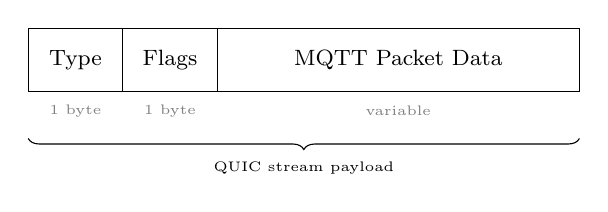
\begin{tikzpicture}[font=\footnotesize]
\draw (0,0) rectangle (7, 0.8);

\draw (1.2,0) -- (1.2,0.8);
\draw (2.4,0) -- (2.4,0.8);
\draw (7.0,0) -- (7.0,0.8);

\node at (0.6, 0.4) {Type};
\node at (1.8, 0.4) {Flags};
\node at (4.7, 0.4) {MQTT Packet Data};

\node[font=\tiny, text=gray] at (0.6, -0.25) {1 byte};
\node[font=\tiny, text=gray] at (1.8, -0.25) {1 byte};
\node[font=\tiny, text=gray] at (4.7, -0.25) {variable};

\draw[decorate, decoration={brace, amplitude=4pt, mirror}] (0, -0.6) -- (7, -0.6)
  node[midway, below=5pt, font=\tiny] {QUIC stream payload};
\end{tikzpicture}
\caption{Flow header format. The 2-byte header replaces MQTT's variable-length fixed header on data streams, where QUIC stream boundaries provide message delimitation.}
\label{fig:flow-header}
\end{figure}

The flow header (Fig.~\ref{fig:flow-header}) consists of two bytes: a type field identifying the MQTT packet type (PUBLISH for data streams) and a flags byte encoding QoS level, retain, and DUP (duplicate delivery). Since the QUIC stream boundary already delimits the message, the two-byte header is sufficient---the receiver reads the type and flags, then parses the remaining stream payload as MQTT packet data without needing MQTT's variable-length framing.

\subsection{Datagram Transport}

As an alternative to stream-based transport, \texttt{mqtt5} supports QUIC datagrams (RFC~9221) for QoS~0 messages. Datagrams bypass QUIC's stream layer entirely: messages are sent as unreliable frames within the QUIC connection, benefiting from QUIC's encryption and connection management but without reliability or ordering guarantees.

Datagram transport is appropriate for latency-sensitive telemetry where occasional message loss is acceptable. Since QUIC datagrams are subject to the connection's congestion window but not to per-stream flow control, they achieve lower latency under loss while maintaining comparable throughput to stream transport (see Section~\ref{sec:evaluation}).

\subsection{Broker Integration}

The client and broker configure their stream strategies independently. On the client side, the application selects a strategy (control-only, per-topic, or per-publish) before connecting; this governs how outbound PUBLISH packets are dispatched onto QUIC streams. On the broker side, a server-wide delivery strategy governs how the broker sends messages to subscribers. In a typical deployment, both sides are configured to the same strategy, but the architecture does not enforce this---a per-topic client can connect to a control-only broker, or vice versa.

The broker mirrors the client's three strategies for outbound delivery to subscribers, maintaining per-connection stream state with LRU eviction to bound stream count. Section~\ref{sec:implementation} details the stream dispatch and receive-side demultiplexing mechanisms.
